%!TEX root = ../../main.tex

\newpage
\chapter{Background}
\label{chapter:background}

In this chapter, we review the background information required to understand the remainder of this thesis.
We draw on several areas of research, such as Information Retrieval (IR) and Natural Language Processing (NLP), and describe how documents are represented and compared, and detail a number of IR measures.
We then give a brief overview of the Topic Detection and Tracking project, and how it related to modern approaches for event detection on Twitter.
Finally, we give a survey of related work in the area of event detection Twitter and describe how it relates to the work presented in this thesis.


\section{Information Retrieval}
Fist we discuss the area of Information Retrieval, and describe some of the most common concepts that we use throughout this thesis.
In a traditional IR task, the goal is to take a query describing some information need, and return a ranked list of documents that are relevant to that query.
In the remainder of this section, we examine some of the basic techniques used to complete this task, and describe how they relate to event detection on Twitter.

\subsection{Document Representation}

One of the most commonly used document and query representations is the Vector Space model \citep{salton1975vector}. The Vector Space model represents both queries and documents as a vector, where each term in the document corresponds to a dimension in the vector.
Terms that occur in a document will have a non-zero value in the vector, while terms that do not appear will have a value of 0.
The Vector Space model is used throughout this thesis to represent documents (tweets).

\subsubsection{TF-IDF}
One of the most common ways of calculating the weight a term has in a vector is known as the Term Frequency-Inverse Document Frequency model, or TF-IDF.
TF-IDF attempts to estimate the importance of a term with regards to both the collection as a whole and document itself.

The TF component is concerned with the weight of the term in relation to the document, the basic premise being that the more frequently a term occurs in a document, the more weight it should carry.
The IDF component, on the other hand, is concerned with the weight of the term in relation to the corpus as a whole.
The IDF component attempts to estimate the amount of information that a term carries on the basis that rare terms should be given more weight as their presence in a document is more likely to be an indication of topic, whilst common terms should be given less weight as they are less topically specific.
TF-IDF is calculated as so:
\begin{displaymath}
	w_{t,d} = \mathrm{tf}_{t,d} \cdot \log{\frac{|D|}{|\{d' \in D \, | \, t \in d'\}|}}
\end{displaymath}
where \(\mathrm{tf}_{t,d}\) is the term frequency of term \(t\) in document \(d\), \(|D|\) is the total number of documents in the collection, and \(|\{d' \in D \, | \, t \in d'\}|\) is the number of documents contain term \(t\).
Note that for retrieval tasks on Twitter, the TF component is often ignored as tweets are very short, and generally do not contain repeated terms.

\subsubsection{Cosine}

Many IR tasks, including event detection, are concerned with the the notion of similarity.
One such similarity measure is cosine similarity, which measures the cosine of the angle between two documents in vector space:
\begin{displaymath}
	\cos{\theta} = \frac{\mathbf{d_1} \cdot \mathbf{d_2}}{\left\| \mathbf{d_1} \right\| \left \| \mathbf{d_2} \right\|}
\end{displaymath}
where \(\mathbf{d_1} \cdot \mathbf{d_2}\) is the dot product of term weighted vectors for the documents, and the norm for vector \(\mathbf{d}\) is calculated as such:
\begin{displaymath}
	\left\| \mathbf{d} \right\| = \sqrt{\sum_{i=1}^n d_i^2}
\end{displaymath}

\subsection{Evaluation Measures}
Throughout this thesis, we use a number of IR standard evaluation metrics, commonly used in IR evaluations.
These measures as based on the concept of relevance.
In IR, relevance is determined based on some information need, usually represented as a textual query.
In event detection, there is no query.
Instead, relevance is defined in relation to an event, either by subjectively evaluating if a cluster of tweets meets some definition of `event', or by matching tweets in the cluster to a pre-determined event in the relevance judgements (represented by a set of tweets).
We discuss this further is chapter \ref{chapter:detection}.

\subsubsection{Recall}

Recall is measured as the fraction of relevant documents that at retrieved from all possible relevant documents. Recall is give as:

\begin{displaymath}
	\text{recall}=\frac{|\{\text{relevant documents}\}\cap\{\text{retrieved documents}\}|}{|\{\text{relevant documents}\}|}
\end{displaymath}

\subsubsection{Precision}
In a traditional IR setting, precision is measured as the fraction of retrieved documents that are relevant to a given query.
For the purpose of evaluating event detection approaches, the lack of a query means that we must consider relevance differently; either in terms of meeting some definition of `event', or by matching back to some event from the relevance judgements.
How this is done is examined in chapters \ref{chapter:collection} and \ref{chapter:detection}.

In a standard IR setting, precision is given as:
\begin{displaymath}
	\text{precision}=\frac{|\{\text{relevant documents}\}\cap\{\text{retrieved documents}\}|}{|\{\text{retrieved documents}\}|}
\end{displaymath}

\subsubsection{F-measure}
Individually, precision and recall show only one aspect of performance.
Perfect recall can be achieved by returning every document in the collection,
whilst perfect precision can be achieved by returning none of them.

F-measure takes both precision and recall into consideration, and combines them into a single score. F-measure ranges between 1 at best (a perfect systems) and 0 at worst. Although it is possible to weight F-measure to prefer precision or recall, the most commonly used F-measure gives equal weight to both, and is the harmonic mean of precision and recall. This is usually called F1 score, and is used throughout this thesis:

\begin{displaymath}
	F_1 = 2 \cdot \frac{1}{\tfrac{1}{\mathrm{recall}} + \tfrac{1}{\mathrm{precision}}} = 2 \cdot \frac{\mathrm{precision} \cdot \mathrm{recall}}{\mathrm{precision} + \mathrm{recall}}
\end{displaymath}

\subsubsection{BCubed}
BCubed Precision and BCubed Recall are similar in theory to the Precision and Recall measures given previously, however BCubed Precision and Recall are calculated for each document or item in the collection, rather than for each category or topic, and are most commonly used for the evaluation of clustering algorithms.
For a given item $e$, BCubed Precision is the proportion of items in the same cluster as $e$ that have the same category as $e$, whilst BCubed Recall represents the proportion of items in the same category as $e$ are in the same cluster as $e$.
Figure \ref{background:graphic:bcubed} illustrates how Precision and Recall for one item, $e$, is computed.

\vspace{0.5cm}
\begin{figure}[h!]
	\centering
	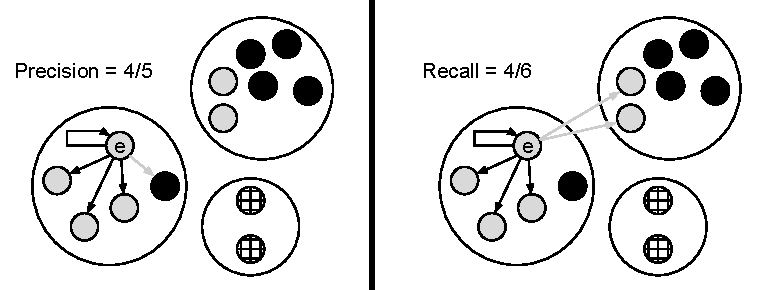
\includegraphics[width=11cm]{Chapters/Background/bcubed.pdf}
	\caption{An illustration of how BCubed Precision and Recall are computed.}
	\label{background:graphic:bcubed}
\end{figure}

Since BCubed Precision and Recall are computed on a per-item basis, the overall Precision and Recall values are taken as the average Precision and Recall values computed over all items.
This is often combined into a single BCubed score using the same F-measure equation as given previously.

\section{Topic Detection and Tracking}
The Topic Detection and Tracking (TDT) project began in 1997, and was a body of research and an evaluation paradigm that addressed the event-based organization of broadcast news \citep{Allan:2002:ITD:772260.772262}.
The motivation behind the project was a system which was capable of monitoring broadcast news and could produce an alert when a new event occurred.

The project was split into five distinct subtasks \citep{Allan:2002:ITD:772260.772262}:

\begin{itemize}
\item \textbf{Story Segmentation} was the task of dividing audio transcripts taken from news shows into individual stories.

\item \textbf{First Story Detection} was the task of recognizing the onset of a new topic (event) in the stream of news stories.

\item \textbf{Cluster Detection} was the task of grouping all stories as they arrived, based on the topics they discuss.

\item \textbf{Tracking} was a task that required systems to identify news stories  discussing the same topic as a set of sample stories, by monitoring the stream of news stories as they appeared.

\item \textbf{Story Link Detection} was the task of deciding whether two randomly selected stories discussed the same topic (event).
\end{itemize}

With the exception of Story Segmentation, the tasks focus on various aspects of document clustering, with the main difference between each task being how it is evaluated.
Of the 5 tasks, First Story Detection (FSD, although often called New Event Detection, NED) was considered the most difficult \citep{Allan:2000:FSD:354756.354843} as an effective FSD system must be effective across all of the tasks to perform well.

Story Segmentation differs in nature from the others as it pertains specifically to a pre-processing step that must be performed before the other tasks can be carried out.
All other tasks work with stories, however the aim of the Story Segmentation task is to detect boundaries between stories automatically using transcripts from the spoken audio of broadcast news shows.
Of all the tasks of the TDT project, Story Segmentation is the least relevant to event detection on Twitter as tweets almost always discuss only a single topic due to their short length.

\subsection{Approaches to TDT}
\label{background:sec:tdt}

At a high level, almost all of the approaches proposed by the TDT project follow the same nearest-neighbour clustering approach shown in algorithm \ref{background:alg:tdt}.
As documents appear in the stream, they are compared to every document that has been seen before (or, if an inverted index is used, than all documents they share a term with), and the similarity between the new document and every other document in the Corpus is calculated.
If one or more similar documents is found (based on some pre-defined threshold), add the new document to cluster containing the closest match, signaling that they discuss the same event.
If no similar documents are found, then a new event has been detected, and a new cluster is formed~\citep{Allan:2000:FSD:354756.354843}.

\begin{algorithm}
	\DontPrintSemicolon
	\KwIn{Minimum similarity threshold $m$}
	index $\gets []$ \\
	clusters $\gets$ [] \\

	\ForEach{document d in the stream} {
		$S(d) \gets \emptyset$ \tcp*{set of documents that share a term with $d$}

		\ForEach{term t in d}{
			\ForEach{document d' in index[t]} {
				$S(d) \gets S(d) \cup d'$ \\
			}
			index[$t$] $\gets$ index[$t$] $\cup$ $d$ \\
		}

		$c_{max} \gets 0$ \tcp*{maximum cosine between $d$ and documents in $S(d)$}
		$n_{d} \gets nil$ \tcp*{document with maximum cosine to $d$}
		\ForEach{document d' in S(d)}{
			$c$ := cosine($d$, $d'$) \\
			\If{$c > c_{max}$}{
				$c_{max} \gets c$ \\
				$n_d \gets d'$
			}
		}

		\eIf{$c_{max} \geq m$}{
			add $d$ to clusters[$n_d$]
		} {
			clusters[d] $\gets$ new cluster($d$) \tcp*{Report d as a new event}
		}

	}
	\caption{A basic TDT approach, similar to that used by UMass and other TDT participants}
	\label{background:alg:tdt}
\end{algorithm}

Unfortunately, the approach shown in Algorithm \ref{background:alg:tdt} does not scale to extremely high volume streams.
The approach takes $O(|D_t|)$ to compute in the worst case, and although the use of an inverted index helps to reduce the average case, it continues to take increasingly longer to process new documents as they are seen.
This has obvious drawbacks when the volume of data is increased from a few thousand documents, to many hundreds of millions of documents per day, which quickly makes this approach computationally infeasible.

This basic model persisted throughout the TDT project, and variations of this model (with efficiency optimizations) are commonly found in event detection approaches for social media \citep{becker2011beyond,Petrovic:2010:SFS:1857999.1858020,Aggarwal12,conf/asunam/OzdikisSO12}.

\subsection{Performance of TDT Systems}
The TDT project produced some reasonably effective systems \citep{UMASS,Yang98,Allan:2005:TTD:1042435.1042899}, however performance was still far below that required for systems to be considered adequate for complete automation \citep{Allan:2000:FSD:354756.354843}.
When the TDT project ended in 2004, research in event detection slowed. It is believed that a plateau had been reached, and that without a radically different approach, the performance of these systems was unlikely to ever improve significantly \citep{Allan:2000:FSD:354756.354843}. This belief has remained true in the context of newswire documents, and many state-of-the-art systems are now over a decade old \citep{UMASS,Yang98,Allan:2005:TTD:1042435.1042899}.
The TDT project was a cornerstone in the development of event detection approaches and is responsible for much of the foundation on which many state-of-the-art event detection approaches for Twitter are based.

\section{Defining an Event}
\label{background:event}
Despite the significant interest and body of work covering the detection and tracking of events, there is little consensus on the exact definition of \textit{event}.
This leads to obvious issues when evaluating and comparing event-based systems, as differences in what is considered an event can make it difficult, or even impossible to compare two systems.

The TDT project defines an \emph{event} as `something that happens at some specific time and place, and the unavoidable consequences'~\citep{Allan:2002:ITD:772260.772262}.
Specific elections, accidents, crimes and natural disasters are examples of events under the TDT definition.
They also define an \emph{activity} as a connected set of actions that have a common focus or purpose.
Specific campaigns, investigations, and disaster relief efforts are examples of activities.
Furthermore, a \emph{topic} is defined as a seminal event or activity, along with all directly related events and activities.
The TDT project dealt with newswire documents, implying a level of significance to the topics being discussed -- it was reasonable to assume that the vast majority of topics in the TDT datasets were significant events.
However this is not the case in Twitter, where a very large portion of documents discuss insignificant personal matters, such as the song a user is listening to.
The TDT project was concerned with the detection of \emph{topics}, the US Presidential Elections is considered a single topic, and stories about the candidates' campaigns, debates, election results, and reactions to the election are all part of the same topic.
There is no distinction made between each of the events within a topic, even though they could occur several days apart.
We believe that this does not make sense in the context of Twitter as discussion moves very quickly and is fixated on the present, unlike newswire documents, which often summarize several days worth of events into a single article.

\cite{Aggarwal12} define a \emph{news event} as being any event (something happening at a specific time and place) of interest to the media.
They also consider any such event (e.g. a speech or rally) as being a single episode in a larger story arc (i.e. a presidential campaign).
They use the term \emph{episode} to mean any such event, and \emph{saga} to refer to the collection of events related within a broader context.

\cite{Becker_beyondtrending} go as far as to define an event in a much more formal, but still subjective manner.
They define an event as a real-world occurrence \(e\) with (1) an associated time period \(T_e\) and (2) a time-ordered stream of Twitter messages, of substantial volume, discussing the occurrence and published during time \(T_e\).
Other definitions, such as that used by~\cite{weng2011event}, define an event simply as a burst in the usage of a related group of terms.

Clearly there is a consensus that events are temporal, as time is a reoccurring theme within all definitions.
However, the consensus appears to end there.
Whilst~\cite{Aggarwal12} and the TDT definition~\citep{Allan:2002:ITD:772260.772262} show a parallel in their hierarchical organization of events (events and topics, news events and sagas), this is less common in other definitions where a distinction between events and topics is not made.
This makes comparisons very difficult; one definition may break an election into many events, while another could consider the election as a single event, or not as an event at all.
Issues are also caused by the subjective nature of what is considered newsworthy.
For example, the definitions used by \cite{weng2011event} and \cite{Becker_beyondtrending} require a substantial number of tweets to discuss a topic before that topic can be considered an event.
This limits the types of topic that can be considered an event to those that generate a substantial volume of tweets, creating a bias towards larger events at the expense of smaller events or those that generate less discussion, such as business or financial news. In Chapter \ref{DefiningEvent} we propose a new definition for `event' that tries to overcome some of these issues.

\section{Event Detection on Social Media}

Analysis of social media has received a lot of attention from the research community in recent years.
However, much of this work focused on blog and email streams  \citep{Zhao:2007:TIF:1619797.1619886,Jurgens:2009:EDB:1859650.1859652,Becker:2010:LSM:1718487.1718524,Nguyen:2011:ERR:2186701.2186707}, using datasets such as the Enron email dataset \citep{citeulike:7616867} or the BlogLines dataset \citep{Sia:2008:ECP:1401890.1401967}.
More recently, the focus has moved towards Twitter due to its popularity with individuals and organizations as a method of real-time broadcast communication, making it interesting to study as a source of information about ongoing real-world events.

\cite{Hu:2012:BNT:2208636.2208672} demonstrated the effectiveness of Twitter as a medium for breaking news by examining how the news of Osama bin Laden's death broke on Twitter. They found that Twitter had broken the news, and as a result, millions already knew of his death before the official announcement.

\cite{Kwak:2010:TSN:1772690.1772751} analyzed the top trending topics to show that the majority of topics (over 85\%) are related to headline news or persistent news. They also found that once a tweet is retweeted, it can be expected to reach an average of 1,000 users.

\cite{WRN2012:osbornebieber} measured the delay between a new event appearing on Twitter, and the time taken for the same event to be updated on Wikipedia. Their results show that Twitter appears to be around 2 hours ahead of Wikipedia. They suggest that Wikipedia could be used as a filter, decreasing the number of spurious events, however at the cost of greatly increased latency. They demonstrate its effectiveness as a filter for their First Story Detection approach \citep{Petrovic:2010:SFS:1857999.1858020}, significantly decreasing the number of spurious events.

\section{Event Detection on Twitter}
A number of excellent survey papers covering Event Detection on Twitter have been published in recent years, including \cite{Hasan17}, \cite{Goswami2016}, and \cite{Atefeh2015}. Rather than replicate their work here, we invite interested readers to refer to these papers for a full survey all event detection approaches for Twitter.
Instead, we survey only the most novel and relevant work in this section.

\cite{sankaranarayanan2009twitterstand} proposed one of the first systems which aimed to detect breaking news and events from tweets. In conjunction with the Twitter garden-hose, they utilize a set of 2,000 handpicked \emph{seeds} -- twitter accounts who primarily post news-related tweets -- that they used as a trusted source of news.
An initial layer of filtering is performed on all incoming tweets, excluding those from the seeds, using naive Bayes classifier trained on a corpus of news and ``junk'' tweets. Next they use an online clustering approach that maintains a list of active clusters, along with an associated TF-IDF \citep{Salton:1988:TAA:54259.54260} feature-vector of the terms used by tweets in the cluster. An incoming tweet is added to a cluster if its similarity with the cluster's feature-vector is above a set threshold, measured using a time-decayed cosine similarity function. An inverted index is maintained so that only active clusters which contain at least some of the terms from the incoming tweet are used for comparison, and clusters with a time centroid greater than 3 days old are marked as inactive and removed from the index.
To further reduce the number of noisy clusters, \cite{sankaranarayanan2009twitterstand} impose an interesting restriction, in that for a cluster to remain active after \(k\) tweets have been added, one of the tweets must come from a seed account.
Despite a number of efficiency optimizations, their approach is unable to scale, or produce results in real-time. Unfortunately, no attempt is made to evaluate the effectiveness of their system other than a small number of empirical observations.

\cite{becker2011beyond} use the clustering approach proposed by \cite{Yang98} as part of the TDT project, and a filtering layer similar to \cite{sankaranarayanan2009twitterstand}.
However, filtering is performed after clustering has taken place, and they attempt to identify likely event clusters, rather than event tweets.
They use a number of features, such as top terms, and number of retweets, to classify clusters as either event or non-event.
Although evaluation of their approach seems to show that it is very effective, it is still based on a model designed for much lower volume streams, and is simply too slow to scale past very small corpora.



\subsection{Locality Sensitive Hashing (LSH) using Random Hyperplanes}
Earlier we discussed how the basic TDT approach as described in Section \ref{background:sec:tdt} could not scale to extremely high volume streams (even with the aid of an inverted index), making it infeasible to use for event detection on Twitter.
\cite{Petrovic:2010:SFS:1857999.1858020} proposed a solution to this using a technique called Locality Sensitive Hashing (LSH).
LSH uses a special hash functions that produce the same hash for documents that are similar, but not necessarily completely identical, allowing documents that are close in vector space to be placed into the same bucket.
Using a set of random hyperplanes and a family of hash functions proposed by \cite{Charikar2002}, the buckets are defined by the subspaces between hyperplanes, such that the probability of similar documents being placed into the same bucket of a hash table is proportional to their similarity.

By using multiple hash tables, each with independently chosen random hyperplanes, the probability of the true nearest neighbour colliding in at least one table can be increased to any desired probability (at the cost of additional computations).
The number of hash tables $L$ needed to give the desired probability of \emph{missing} a nearest neighbour $\delta$ can be computed as:
\begin{displaymath}
	L = log_{1-P^k_{coll}} \delta
\end{displaymath}
where $k$ is the number the number of hyperplanes, $P_{coll} = 1-\frac{\theta(x,y)}{\pi}$ where $\theta(x,y)$ is the expected angle between similar documents $x$ and $y$.
Petrivic et al. use values of $k = 13$, $\theta(x,y) = 0.2$ and $\delta = 0.025$ to compute $L$, values which we also use when replicating their work in Chapter \ref{chapter:collection}.

\subsubsection{Variance Reduction}
Although the use of LSH improves computational efficiency, it proves to be considerably less effective than the standard TDT approach.
This is because LSH is most effective when the true nearest neighbour is very close (i.e. has a high similarity) to the query document.
If the nearest neighbour is far from the query document, then LSH often fails to find it.
To overcome this, \cite{Petrovic:2010:SFS:1857999.1858020} use a `variance reduction' strategy when a nearest neighbour is not found using LSH.
In these instances, the approach falls back the traditional TDT model, and uses an inverted index to retrieve a list of documents to search for a nearest neighbour.
However, unlike the basic TDT model, a limit is placed on the number of documents searched, and only the most recent 2000 documents returned from the inverted index are compared.
This helps to improve the effectiveness, and brings it inline with that of the basic model, whilst still being considerably more efficient.

\subsubsection{Additional Efficiency Enhancements}
Since the number of buckets is limited, in a streaming scenario where the number of documents in unbounded, the number of documents in each bucket will continue to grow as new documents are processed.
This would require an unbounded amount of space and the number of comparisons made would also grow for each new document, eventually making even the LSH approach infeasible.
To overcome this, \cite{Petrovic:2010:SFS:1857999.1858020} limit the number of documents in a bucket to a fixed number based on the expected number of collisions, which can be computed as $n/2^k$ where $n$ is the total number of documents and $k$ is the number of hyperplanes used.
When a bucket is full, the oldest document in the bucket is removed from that bucket (and only that bucket) to make room for new documents.
Due to the use of multiple independent hash tables, the removal of the document from a bucket does not prevent it from being retrieved from other hash tables, although eventually all documents are removed from all hash tables.

To keep the number of comparisons per document fixed, similarity comparisons are performed for at most $3L$ documents (where $L$ is the number of hash tables).
The documents are selected by counting the number of times a document collides across the $L$ hash tables, and taking the top $3L$ documents with the most collisions.

\subsubsection{Cluster Ranking}
Although the use of LSH improves computational efficiency and allows the application of a TDT approaches on Twitter-scale data, it does not address the issue of noise and spam, which is found in excess on Twitter but is not present in the TDT datasets.

\cite{Petrovic:2010:SFS:1857999.1858020} investigated a number of ranking approaches for ranking clusters produced by their system.
They found that ranking clusters by the number unique users was more effective than the raw number of tweets.
They also found that the amount of information contained in the thread, measured using Shannon entropy \citep{Shannon:2001:MTC:584091.584093}, was a good indicator of quality.
Shannon entropy, $H$, is measured as:
\begin{displaymath}
	H = -\sum_i{\frac{n_i}{N} \log \frac{n_i}{N}}
\end{displaymath}
where $n_i$ is the number of occurrences of term $i$ in a cluster,	and $N = \sum_i{n_i}$ is the total number of all term occurrences in the cluster.
Clusters with a low entropy, defined as $H < 3.5$ by Petrović et al., are moved to the bottom of the ranking -- effectively marking them as noise.
This entropy based approach to removing noise and spam works because it helps to filter out automated ``bot'' content, where the same message is published by many different accounts in an automated manner.
Clusters where the content shows very little or no variation will have a relatively low entropy (information content), whereas clusters that show more variation (due to having different sources and authors) will have a higher entropy and contain more information.
By combining both the unique user counts and entropy based filters, \cite{Petrovic:2010:SFS:1857999.1858020} are effectively requiring a topic to be discussed by a broad range of users for it to be considered an event.

Note that this ranking approach requires either a fixed period to have elapsed or a set number of tweets to be processed before the ranking can be made.
For example, the ranking may be updated once per hour, or once every 100,000 tweets.
This takes away from the usefulness of the approach in a real-time scenario, making it more batch-based than real-time.

\subsection{Efficient Clustering Using a Fixed Number of Clusters}
If documents are restricted to a single cluster, an easy efficiency gain can be found by comparing new documents to existing clusters (rather than every other document).
Since the number of clusters will always be smaller than the number of documents, fewer comparisons are needed to find the nearest neighbour cluster.
This approach was used by \cite{Aggarwal12}, with the additional constraint that the number of clusters (usually several hundred) is kept constant, ensuring linear complexity (i.e., the time taken to process each new document is a constant).
An overview of their clustering approach is given in Algorithm \ref{background:alg:sbs}.

\begin{algorithm}
	\DontPrintSemicolon
	\KwIn{Number of clusters $k$}
	clusters $\gets$ [$k$] \\
	$i, \mu, \sigma, M_0, M_1, M_2 \gets$ 0 \\

	\ForEach{document d in the stream} {
		$s_{max} \gets 0$ \tcp*{maximum similarity between $d$ and all clusters}
		$n_{c} \gets nil$ \tcp*{cluster with maximum similarity to $d$}
		\ForEach{cluster c in clusters}{
			$s$ $\gets$ similarity($d$, $c$) \\
			\If{$s > s_{max}$}{
				$s_{max} \gets s$ \\
				$n_c \gets c$
			}
		}

		\eIf{$s_{max} < \mu -3 \cdot \sigma$}{
			replace most stale cluster with new cluster containing $d$
		} {
			add $d$ to clusters[$n_c$]
		}

	update $M_0, M_1, M_2$ additive \\
	$\mu$ $\gets$ $M_1/M_0$ \\
	$\sigma$ $\gets$ $\sqrt{M_2/M_0-\mu^2}$

	}
	\caption{A clustering approach as given by \cite{Aggarwal12} with a fixed number of clusters}
	\label{background:alg:sbs}
\end{algorithm}

\subsubsection{Identifying Event Clusters}
\cite{Aggarwal12} define two ways that a new event can occur using their clustering approach:
\begin{itemize}
	\item \emph{novel} events, which are caused by the creation of a new cluster containing only a single document (thus, also requiring the removal of a ``stale'' cluster)
	\item \emph{evolution} events, where a cluster experiences a rapid increase in the relative volume of documents it receives due to the emergence of a new topic
\end{itemize}

New clusters (\emph{novel} events) are created when a nearest neighbour cluster cannot be found among the existing clusters.
Unlike most event detection and TDT systems, \cite{Aggarwal12} use an adaptive similarity threshold based on the Three Sigma rule \citep{Pukelsheim94}, which states that the expected similarity value should be within 3 standard deviations of the mean similarity across all previously seem documents.
For use as a minimum threshold for similarity, only the lower bound is used:
\begin{displaymath}
	threshold = \mu - 3 \cdot \sigma
\end{displaymath}
where $\mu$ is the mean and $\sigma$ is the standard deviation of all similarity measures that have been seen before.

To compute the $\mu$ and $\sigma$ values efficiently, \cite{Aggarwal12} use the first 3 moments of the set of highest similarity scores $S$ (i.e., the set of  similarity score of each document to its nearest neighbour cluster):
\begin{align*}
	M_0 &= \sum_{i = 0}^{|S|}{S_i^0} & M_1 &= \sum_{i = 0}^{|S|}{S_i^1} & M_2 &= \sum_{i = 0}^{|S|}{S_{i}^2}
\end{align*}
These values can be updated as each new document is clustered, and used to calculate the $\mu$ and $\sigma$ as show in Algorithm \ref{background:alg:sbs}.

If a document has a highest similarity score below $\mu - 3 \cdot \sigma$ then a new cluster is created and the document is added to it.
Since this approach requires a constant number of clusters for linear time complexity, the creation of a new cluster requires the removal of an existing cluster.
\cite{Aggarwal12} opt for the simplest approach in this case, and remove the cluster which has not had a document added for the longest period of time.

An \emph{evolution} event is said to have occurred when the fraction of documents added to a cluster during time $t_{i}$ is greater than the fraction added during period $t_{i-1}$ by a factor of $\alpha$.
For a cluster $c$, during time periods $t_i$ and $t_{i-1}$, an evolution event occurs if:
\begin{displaymath}
	\frac{F(c, t_i)}{F(c, t_{i-1})} \geq \alpha
\end{displaymath}
where $F$ gives the fraction of all documents during time $t$ that were added to cluster $c$.
Evolution events are necessary to capture real-world events that are similar enough to an existing cluster that they do not cause a new cluster to be created.
The change in relative volume of documents represents a change in behavior which can be seen as an indicator of a new event.

\subsection{Supervised Approaches to Event Detection}
\cite{Sakaki:2010:EST:1772690.1772777} were concerned with the detection of specific types of event, in particular, earthquakes and typhoons, with the aim of issuing alerts to those in the path of these disasters. Their approach, although simple, is very effective. They specify a set of predefined keywords which are associated with the type of events they are trying to detect (e.g. earthquake, shake, cyclone, typhoon, etc.,). They monitor an incoming stream of tweets for these keywords, and for each tweet found, they classify it using a Support Vector Machine (SVM) as either event-related or not. If they find enough event-related tweets in a short period of time, then their systems decides that the event is real, and issues alerts to those who could be affected. Despite the effectiveness of their approach, there are obvious drawbacks. Firstly, it can only detect specific types of event, and secondly, it requires training data for each of the types of event we want to detect.

\subsection{Natural Language Approaches}
\cite{Choudhury11extractingsemantic} examined how linguistic features and  background knowledge could be used to detect specific types of sports events with high precision. However their approach requires significant domain knowledge of the sporting events and large amounts of manual labeling to prepare a classifier for each specific type of event, making it difficult and time-consuming to generalize.

\cite{Ritter:2012:ODE:2339530.2339704} used named entities, ``event phrases'' and temporal expressions to extract a calendar of significant events from Twitter.
However, their approach requires that tweets contain temporal resolution phrases, such as ``tomorrow'' or ``Wednesday'' for their approach to resolve between an entity and a specific time.
This means that smaller events, which do no generate much discussion before they happen, are unlikely to be detected. Additionally unexpected events, which are often the events which are of most interest, are unlikely to be detected as they will be discussed as they happen, and without any temporal resolution phrases.

Most similar to our work is that of \cite{Reuters2017}, who use a partitioning technique to efficiently cluster documents by splitting the tweet term space into groups they call `semantic categories', such as named entities, mentions, hashtags, nouns and verbs.
To ensure that only novel events are reported, they compare each new event to old events, filtering out any events that have already been reported.
They merge events by comparing the top 20\% of entity terms, based on term frequency, which reduces event fragmentation.
They evaluate their approach using the Events 2012 corpus we create in chapter \ref{chapter:collection}, finding that their approach outperforms the LSH approach when measured using NMI and B-Cubed cluster performance metrics.
Although this approach outperforms their baseline approach, the LSH approach of \cite{Petrovic:2010:SFS:1857999.1858020} using their chosen evaluation metrics, they do not report precision or recall values, making it difficult to compare directly.

\subsection{Burst and Trend Analysis}

\section{Differences between Event Detection and other IR Tasks}
\label{background:sec:diffs}
Despite being viewed as an IR task, Event Detection has a number of characteristics that differ from more common IR tasks.
The most obvious of these is the lack of a user-provided query.
Rather than searching for documents relevant to a specific query, event detection systems first must detect new events and track which documents belong to the same topic.
This means that the notion of relevance is much more ambiguous, and creates a number of issues with the evaluation of event detection approaches.

\section{Test Collections}
Ir order to fairly and accurately evaluate Information Retrieval systems of any kind, a standard test collection and set of relevance judgements are required.
The majority of modern test collections are created using a pooling approach, where a set of topics or queries are selected and used to retrieve documents from a number of different systems.
The union of the top \(n\) documents per topic, taken from each system systems, is then used create a pool of documents for each topic.
Each document in the pool is then judged to be relevant or non-relevant to the topic, and documents which are not in the pool are assumed to be non-relevant.

This pooling  approach is commonly used to generate relevance judgements for collections provided to researchers participating in conferences such as the Text REtrieval Conference (TREC), which is sponsored by the National Institute of Stands and Technology (NIST) in the United States.
Researchers are first given the test collections with a set of pre-selected topics, and are asked to submit the results from their retrieval systems to experts who then perform the pooling and annotate the documents.
Given the scale of modern test collections, this can be a slow and expensive undertaking, which restricts the number of ``tracks'' (a set of tasks focused on some facet of a retrieval problem) that can be run each year, and thus limits how many test collections and relevance judgments can be created this way.

More recently, crowdsourcing has become a popular method of cheaply and quickly generating relevance judgements since it does not rely on the timing of particular conferences or and does not require experts to gather relevance judgements.
\cite{Alonso:2008:CRE:1480506.1480508} describe how crowdsourcing can be used to gather relevance judgements and discuss their crowdsourcing methodology called `TERC', which they find provides fast turnarounds whilst being low cost and producing high quality results.
However, they also describe some of the issues and limitations which need to be addressed, such as the need for strict quality control and the `artificiality' of the task.
Whilst they propose some solutions to these issues, they recognize that many of the solutions are domain specific, and not applicable in all situations.

Issues remain with the pooling method itself.
\cite{Buckley:2007:BLP:1298708.1298735} highlighted a number of issues associated with pooling when dealing with large collections, and showed that standard pooling techniques can introduce bias when dealing with large collections.
They make a number of suggestions, such as engineering the topics or forming pools differently, that could reduce bias and allow for the creation of large unbiased test collections using pooling.
However, the use of pooling to create a test collection for event detection poses additional challenges which require more substantial changes to the TREC-style pooling methodology than those proposed by \cite{Buckley:2007:BLP:1298708.1298735}.

\subsection{The Pooling Approach and Event Detection}
As discussed in section \ref{background:sec:diffs}, there are no pre-defined topics or queries for event detection systems to use.
Rather, systems aim to automatically \emph{discover} a sub-set all all topics being discussed in the collection that meet the criteria for being an \emph{event} (as we will discuss in Chapter \ref{chapter:collection}, defining these criteria is not straightforward).
A perfect system would detect all documents for each event being discussed, however in practice, different event detection approaches discover different events.
This makes it impossible to pool the results from event detection approaches using a TREC-style pooling methodology since it is not obvious what the various topics are or how they should be merged to create the pools for judgment.

Even if it was possible to identify and pool tweets for each of the topics, event detection systems generally do not produce a rank for each tweet, instead relying on their temporal order.
Temporal order is a natural and useful way of ordering tweets that discuss real-world events, as events are often discussed in real-time.
Since this does not infer any sort of quality or usefulness score from the system, there is no way of identifying the top $n$ documents from each event from each system, making it difficult to efficiently pool them for judgment.

\subsection{Twitter Corpora}
\label{background:sec:twittercorpora}

\begin{table}[b]
	\centering

	\caption[A comparison of the different Twitter corpora available prior to Events 2012 corpus.]{A comparison of the different Twitter corpora available prior to this collection. Values marked with * are estimates as exact numbers are not given. A question mark (?) indicates that the number of events is not clear.}
	\label{table:collectionsCompared}

	\begin{tabulary}{\textwidth}{lccccc}

	\toprule
	\textbf{Collection} & \textbf{Period} & \textbf{Tweets} & \textbf{Event based} & \textbf{Events} & \textbf{Unbiased} \\
	\midrule

	\cite{McCreadie:2012:BRT:2348283.2348495} & 14 days & 16M & No & - & - \\
	\cite{Becker:2012:ICP:2124295.2124360} & 28 days* & 2.6M & Yes & ? & No \\
	\cite{Petrovic:2012:UPI:2382029.2382072} & 75 days* & 50M & Yes & 27 & No \\
	\textbf{This Work} 	& 28 days & 120M & Yes & 506 & Yes \\

	\bottomrule
	\end{tabulary}

\end{table}

A broad range of Twitter collections have been created for various tasks, however the majority of these lack relevance judgements or are simply collections of tweets that contain specific words or hashtags.
There have been very few attempts to create large-scale, robust test collections containing a wide range of topics with relevance judgments.
Table \ref{table:collectionsCompared} shows the most noteworthy and relevant Twitter corpora, compared to the collection we describe the creation of in Chapter \ref{chapter:collection}.

TREC utilized the pooling approach to gather relevance judgements in 2011 and 2012 as part of the Microblog Track.
An ad-hoc retrieval task was used both years on the Tweets2011 \citep{McCreadie:2012:BRT:2348283.2348495} collection, across 100 queries (50 each year).
The collection was the first publicly available, large-scale, Twitter corpus, consisting of a random sample of 16 million tweets collected over a period of 2 weeks in 2011.

The Tweets2011 corpus contains tweets in all languages, however queries and judgements were only made using English language tweets, of which there are approximately only 4 million in the corpus.
Furthermore, the topics and relevance judgments  were designed specifically for ad-hoc retrieval (one example query being `fishing guidebooks'), meaning that the relevance judgements are unsuitable for event-based analysis.
The TREC Microblog Track also ran in 2013, however the track moved to an experimental track-as-a-service approach, where the corpus was hosted by TREC and participants had to be queried using an API.
The only way to obtain tweets from the collection was to query the API for specific keywords, making it impossible to process the corpus as a time-ordered stream.
Once again, the set of topics used were designed specifically for ad-hoc retrieval, making them unsuitable for event-based analysis.

\cite{Becker:2012:ICP:2124295.2124360} produced what we believe was the first Twitter collection of events.
Their collection contains 2.6 million tweets posted by users from New York,
however this limits its usefulness for the evaluation of event detection systems as it limits the types of event that can be detected.
The small size of the corpus also limits its usefulness.
The 2.6 million tweets represents just ~0.02\% of the volume of tweets posted to Twitter over the 28 day period that the collection covers, meaning that it does not give a true representation of the scale found on Twitter.

\cite{Petrovic:2012:UPI:2382029.2382072} created a corpus designed to evaluation the First Story Detection task of the TDT project.
While their collection contains a relatively high 50 million tweets from the beginning of July until mid-September 2011, they gathered judgments for only 27 events.
The small number of events is not a problem for the evaluation of First Story Detection, a sub-task of event detection, where the aim is to detect the first story discussing a new event.
However, it does prevent the collection from being used to evaluate event detection, since missing any of the 27 events will have a large impact on measured performance, and any differences between systems will likely not be statistically significant due to the small sample size.

Although these collections have been made available, albeit in a limited fashion, none appear suitable for the analysis of events and comparison of event detection approaches.
The collection produced by~\citeauthor{Becker:2012:ICP:2124295.2124360} is simply too small to be of practical use for event detection, while the collection created by~\citeauthor{Petrovic:2012:UPI:2382029.2382072} covers too few events for a fair comparison to be made.
One reason for the lack of comparative corpora may be the difficulty and expense of creating one.
A reasonable sized Twitter corpus will contain tens of millions of documents -- performing a manual search on corpus of that magnitude is simply impossible.
To overcome this,~\citeauthor{Petrovic:2012:UPI:2382029.2382072} used a procedure similar to NIST, where expert annotators (primarily the authors of the paper) read the description of an event and used keywords to search for relevant documents.
However, this approach means that events (i) must be carefully identified in advance (potentially introducing bias) (ii) annotation requires expensive and slow experts, and (iii) it does not scale well past a certain size (\citeauthor{Petrovic:2012:UPI:2382029.2382072} were only able to create judgements for 27 events).

\subsection{A New Approach}
Issues with both TREC-style pooling and crowdsourcing, as well as the lack of an unbiased and comparable test collections for event detection, highlights the need for a new methodology that can be used for the creation of large-scale test collections for event detection on Twitter.
A new pooling approach is needed to cope with the lack of predefined topics and document ranking, whilst new crowdsourcing techniques are needed which maintain the fast turnarounds and low-cost associated with crowdsourcing, but ensure high-quality results.

